\documentclass[letterpaper,10pt]{article}
\usepackage[top=2cm, bottom=1.5cm, left=1cm, right=1cm]{geometry}
\usepackage{amsmath, amssymb, amsthm,graphicx}
\usepackage{fancyhdr}
\pagestyle{fancy}

\lhead{\today}
\chead{Regression 4.1b}
\rhead{Justin Hood}

\newcommand{\Z}{\mathbb{Z}}
\newcommand{\Q}{\mathbb{Q}}
\newcommand{\R}{\mathbb{R}}
\newcommand{\C}{\mathbb{C}}
\newtheorem{lem}{Lemma}

\begin{document}
We consider the following model of the data,
\[Y=\beta_0+\beta_1X_1+\beta_2X_2+\epsilon\]
For the sales data, we have,
\[Y=29.3468+5.6128X_1+3.8344X_2\]
\begin{enumerate}
\item We begin by plotting each of the independent variables against the Sales data in order to determine the nature of their relationship.\\
\begin{center}
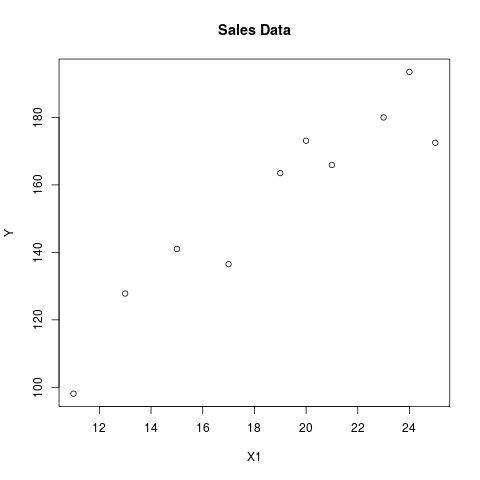
\includegraphics[scale=.5]{yx1.png}
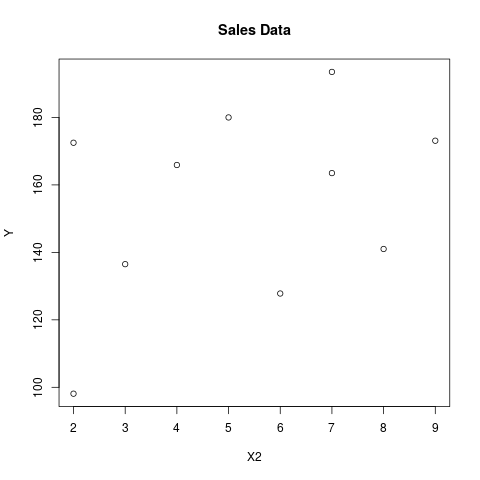
\includegraphics[scale=.5]{yx2.png}
\end{center}
We see from these plots that $X_1$ is clearly linearly related to $Y$, while the relationship between $X_2$ and $Y$ is more complex than a simple linear relationship. We consider the model, $\beta_0+\beta_1X_1+\beta_2X_2+\beta_3X_2^2+\epsilon$ Computing, we find our model to be,
\[Y=19.0737+5.5596X_1+9.2229X_2-.5129X_2^2\]
\item We next consider a model that accounts for potential interactions between $X_1$ and $X_2$, $\beta_0+\beta_1X_1+\beta_2X_2+\beta_3X_2^2+\beta_4X_1X_2+\epsilon$. We compute this model to be,
\[Y=27.43798+5.08130X_1+7.28995X_2-.53110X_2^2+.11473X_1X_2\]
\item In order to test the significance of this interaction model, we shall test,
\begin{align*}
H_0&: \beta_4 = 0\\
H_A&: \beta_4 \neq 0
\end{align*}
The $p$-value for our computed value of $\beta_4$ is $.014032$. Thus, at $\alpha=.05$, we may accept that there is a non-zero level of interaction between the variables. At the $\alpha=.01$ level however, we see that the interaction is not significant enough.
\item We now compare the $R^2$ value for each of the computed models,
\begin{center}
\begin{tabular}{c|c|c}
Model & $R^2$ & Adjusted $R^2$ \\\hline
1 & $0.9901$ & $0.9873$ \\
2 & $0.9975$ & $0.9962$\\
3 & $0.9993$ & $0.9988$
\end{tabular}
\end{center}
We see that as we have added a term to each of these models, the overall ``correctness" of the successive models increases. Thus, we may conclude that Model 3 is the best overall at predicting the data.
\item Finally, we consider predicting the sales price(in thousands) using the inputs, $X_1=16$ and $X_2=8$. The results for each model are below,
\begin{center}
\begin{tabular}{c|c|c}
Model & Point Prediction & 95\% Interval\\\hline
1 & $149.83$ & $(141.17,\ 159.48)$ \\
2 & $148.98$ & $(144.07,\ 153.90)$ \\
3 & $147.75$ & $(144.70,\ 150.81)$
\end{tabular}
\end{center}
We note that each sucessive prediction interval is smaller than the last, implying that these models are sucessively more accurate than the last.
\end{enumerate}
\end{document}
